\section{Introduction}
\label{sec:introduction}
Recent advancements in machine learning (ML) have notably enhanced models' capabilities to extract valuable information from images. This is particularly relevant for indoor positioning systems (IPS) with extended capabilities to detect falls or signals for help. Traditionally, various non-visual sensors such as wearable devices, passive infrared sensors (PIR), radio-frequency identification (RFID), and light detection and ranging (LIDAR) have been utilized in IPS. These technologies preserve privacy effectively as they are mostly incapable of identifying personal data. However, for future applications requiring detailed context and capabilities, these sensors fall short where visual sensors excel.

The emergence of automated \textit{on-device} processing marks a significant progression in privacy preservation of visual sensors in IPS. With on-device processing, images no longer need to be analyzed manually or transmitted over the internet, allowing for the creation of more advanced and comprehensive systems. As highlighted by \citeauthor{s22218119}, integrating indoor positioning systems (IPS) with human activity recognition (HAR) is essential to detect incidents like falls or injuries, especially among elderly individuals living alone (\citeyear{s22218119}). 

This thesis explores the development and deployment of a privacy-preservant person locatization system, particularly advocating for on-device processing to mitigate privacy concerns. As part of the on-device processing, sensitive data, such as images, are either deleted or obfuscated immediately after inference, complicating analysis validation but significantly enhancing privacy.

Typically, machine learning models for person detection are pretrained on large, generic datasets and validated on similar datasets, which may not accurately represent specific deployment scenarios. This thesis addresses this gap by collecting a specialized dataset in a typical dark-lit indoor museum/aquarium setting and evaluating various detectors fine-tuned to this environment. A month-long live experiment was conducted at the Fisheries and Maritime Museums (FIMUS) aquarium to assess these systems' real-world applicability. During this experiment, some images were blurred and retained to verify the model's inferences, enhancing our understanding of their practical utility and limitations.

Figure \ref{fig:example_from_aquarium}a displays an example image from the collected FIMUS dataset, while Figure \ref{fig:example_from_aquarium}b shows an image from the live experiment that was kept for verification purposes.
\begin{figure}[H]
    \centering
    \begin{subfigure}{0.475\textwidth}
        \centering
		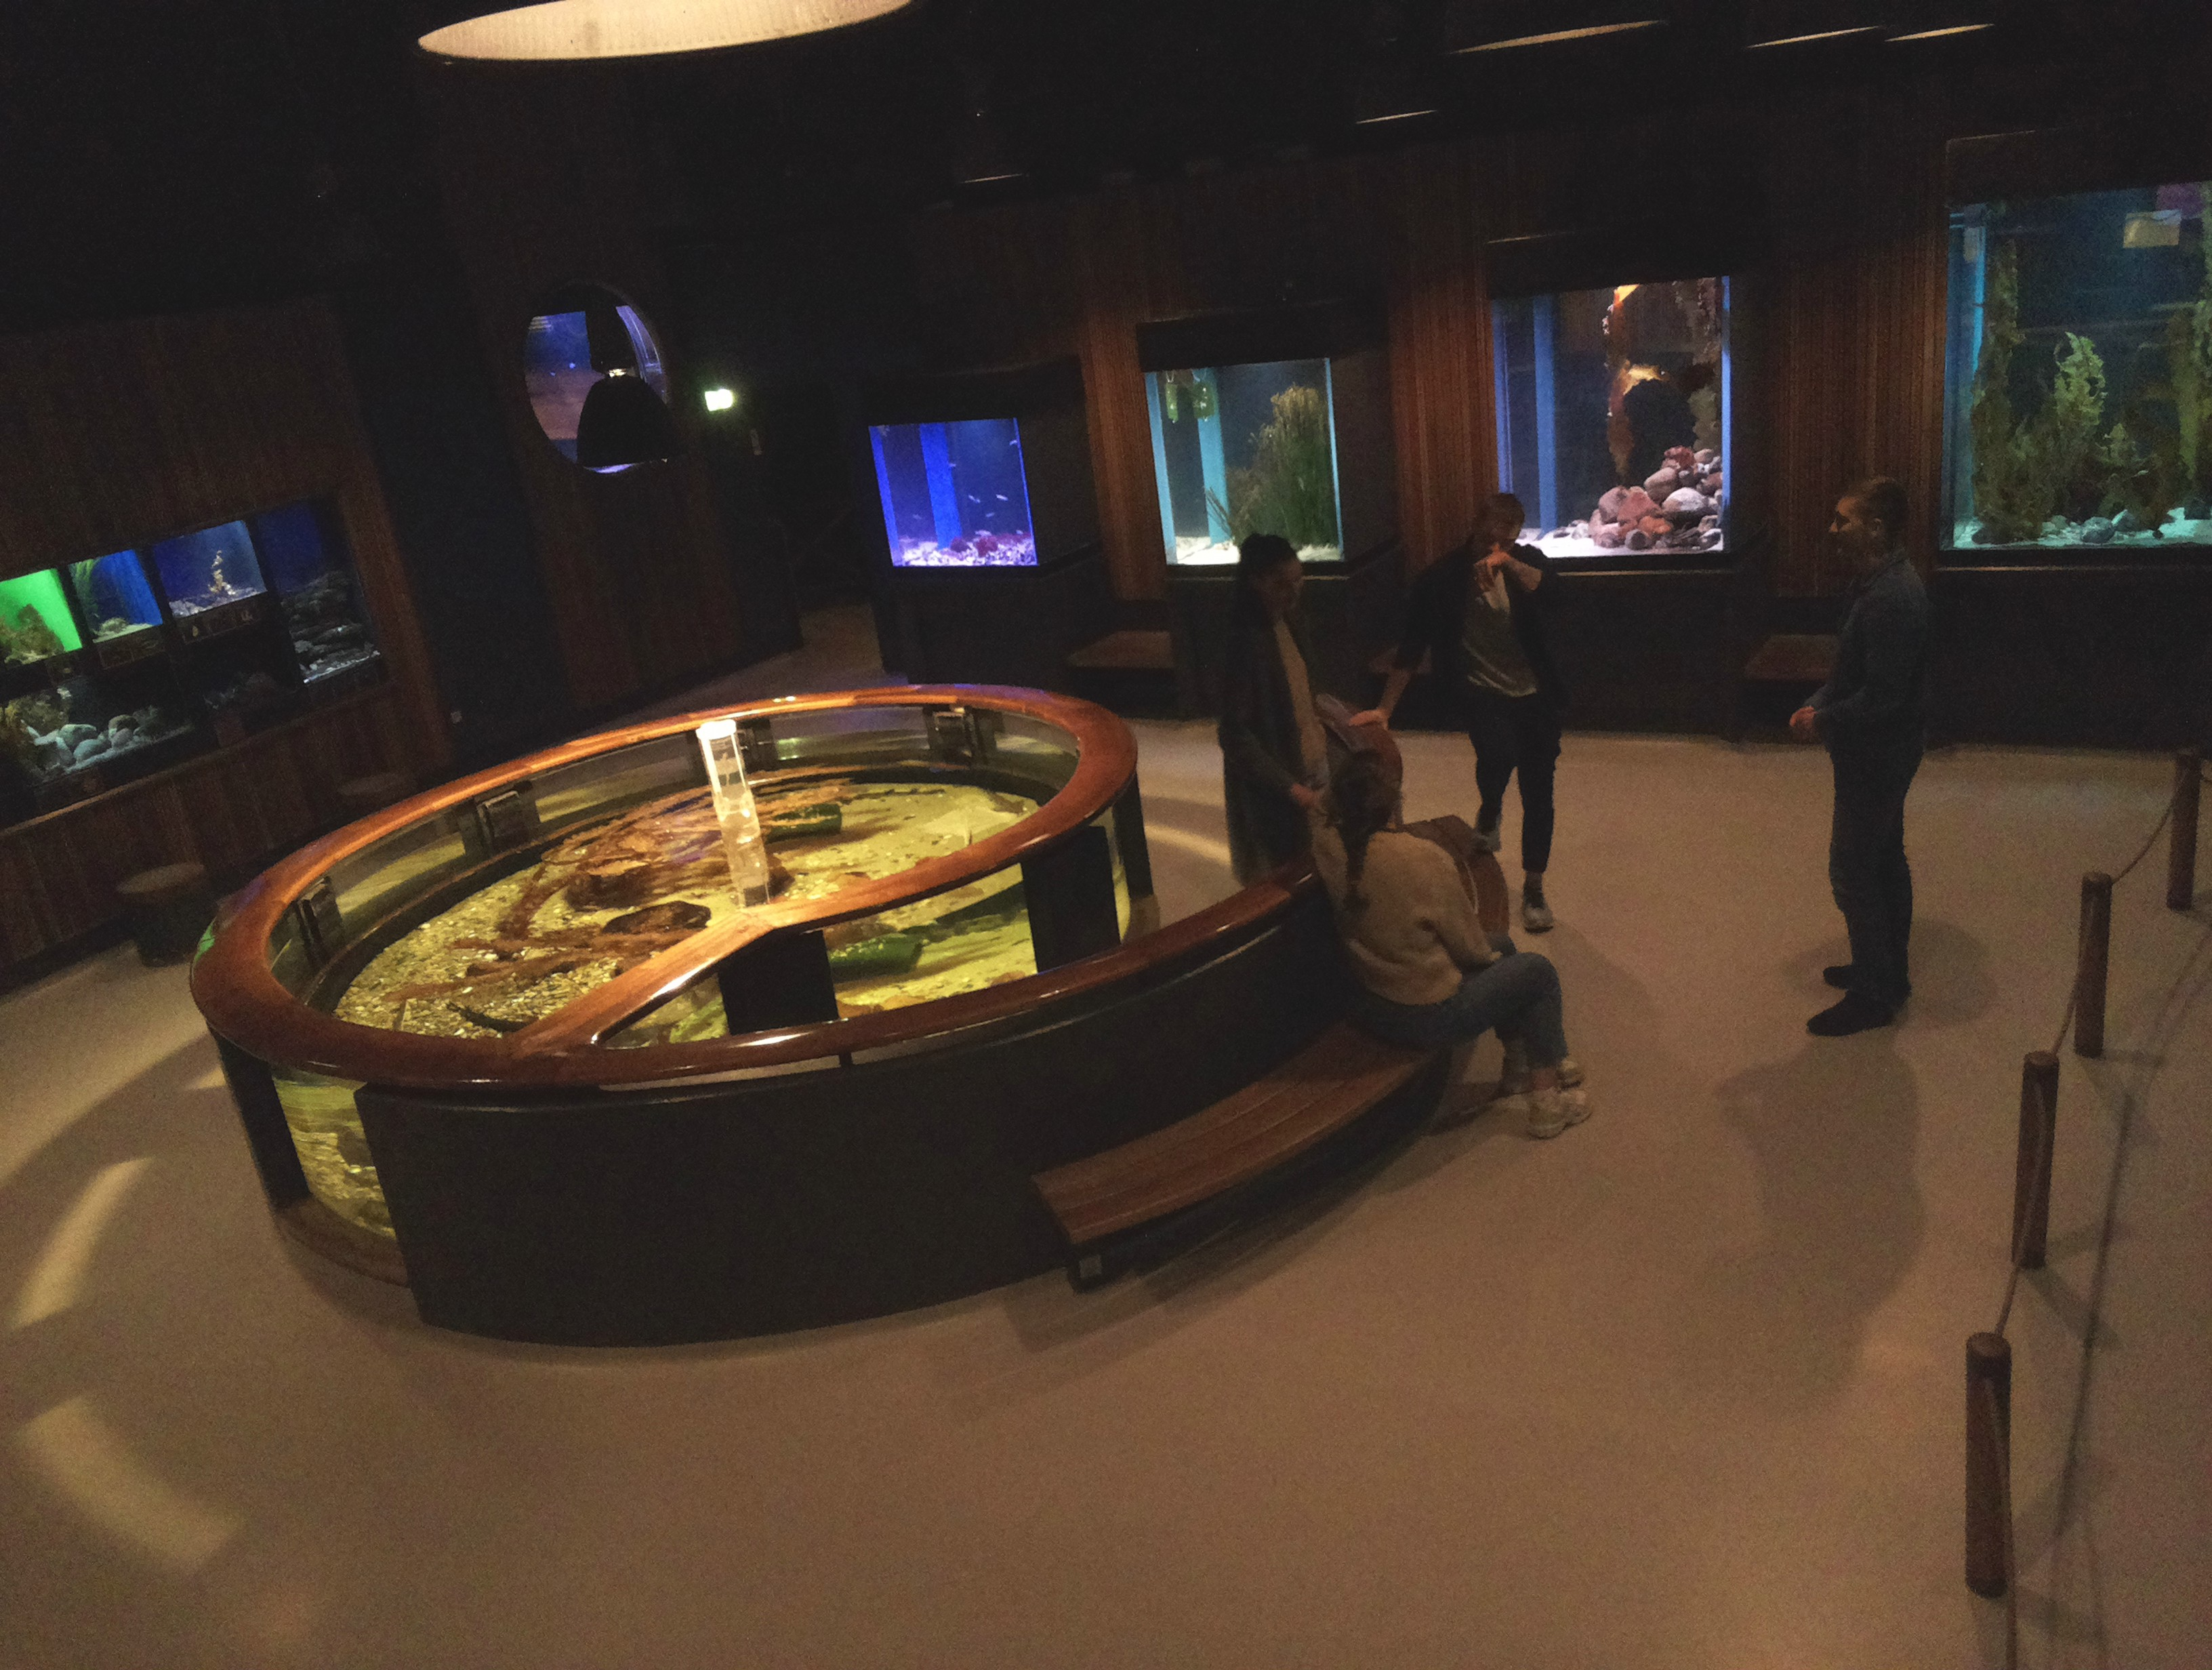
\includegraphics[width=\textwidth]{Images/DeviceImages/2nd-iteration/example.jpg}
        \caption{Example Image From the FIMUS Dataset.}
    \end{subfigure}
    \hfill
    \begin{subfigure}{0.475\textwidth}
        \centering
        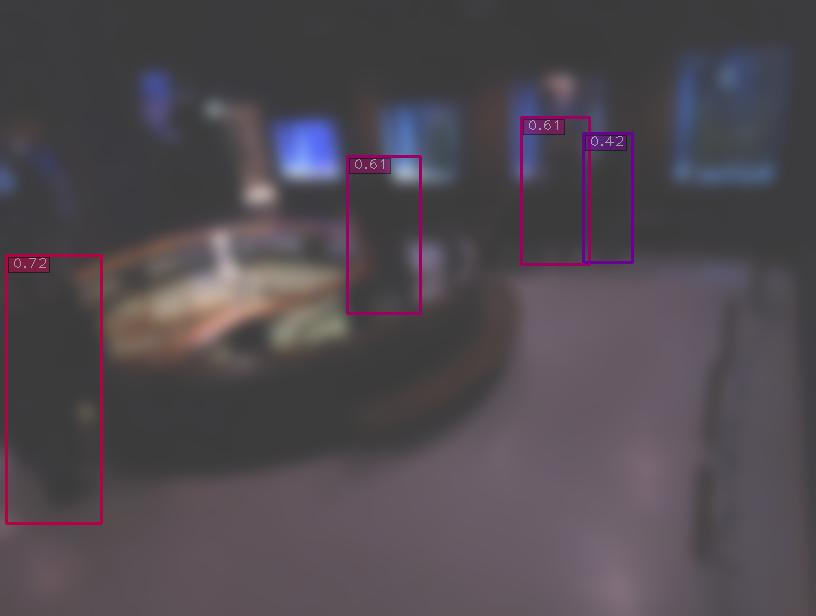
\includegraphics[width=\textwidth]{Images/DeviceImages/live-example.jpg}
        \caption{Example Image From the Live Detections.}
    \end{subfigure}
	\caption{Images From The Fisheries and Maritime Museum (FIMUS)}
	\label{fig:example_from_aquarium}
\end{figure}

\newpage
\subsection{Problem Description}
\label{sec:problem_description}
Recent advancements in computer vision and machine learning have transformed the field of person localization in public spaces. Traditionally, surveillance systems rely on centralized processing, where video feeds are sent to a remote server for analysis. This method poses significant privacy risks as it exposes sensitive information to potential interception during transmission. This thesis advocates for a shift towards \textit{on-device} processing, where analytics are performed locally on edge devices, thus enhancing privacy by eliminating the need to transmit raw video data. Another aspect of on-device processing is to algorithmically analyze the video feed by the use of machine learning, instead of humans.

Additionally, the efficacy of object detection models is commonly measured using generic datasets like COCO, which may not accurately represent the specific conditions and image characteristics of a real-world deployment environment. Such discrepancies can result in models performing suboptimally in actual settings, where variables like lighting, camera angle viewpoint, scale, rotation, and object occlusion play crucial roles. The quality and relevance of the data used to test and train a model for deployment should be as similar to the deployment scenario as possible. However, assessing the impact of dataset relevancy and quality on model accuracy presents substantial challenges, with limited research available on this subject. Consumers are thus left in the dark by the researchers in the field with regards to how much effort should be put into finding the best suited test dataset for model testing and fine-tuning.


\subsection{Scope}
\label{sec:scope}
To demonstrate the feasibility and effectiveness of on-device person localization, two devices were deployed at the \textit{Fisheries and Maritime Museum}\footnote{In original language: Fiskeri og Søfartsmuseet} (FIMUS) aquarium in Esbjerg, Denmark. The indoor, low-light conditions of the aquarium presented specific challenges that the deployment aimed to address. The deployment camera angle viewpoint on the persons in the area was different than most images in the COCO dataset that the models were pre-trained on. For this reason, a dataset consisting of 3,397 images was collected and labeled, providing a foundation for fine-tuning several object detector models to better fit the deployment scenario, and to investigate the impacts of dataset relevancy on the model performances. The dataset was collected using varying and fixed camera configurations, creating a dataset capable of investigation of data quality (different camera configurations) on the model accuracies. Figure \ref{fig:example_from_aquarium} showcases an example image from this dataset. During the final month of the project, a device was deployed to anonymously and automatically detect the positions of persons\footnote{\textit{People: Where individual persons, or a number of such, are intended, this word should be discarded in favor of persons.(\cite{vizetelly2015deskbook}).}} in the room every 2 minutes during opening hours. The data was visualized through heatmaps and bar charts of peak visitation times of the day. 

The scope of this thesis is twofold: firstly, the thesis details a demonstation of the implementation of a privacy-preserving person localization system; secondly, the thesis assesses the validity of object detection model performances across general and specific datasets to evaluate the real-world impacts of scientific advancements. This dualistic approach not only highlights the practical application of privacy technologies in object detection but also investigates how different data environments affect model efficacy.

The inclusion of a previously implemented system serves as a practical foundation for this thesis, shortening the theoretical to practical implementation pathway. By utilizing the images from the specific deployment scenario, thus specializing our solution to the problem, the thesis project aims to achieve superior results at the expense of reduced generalizability. However, the general nature of the thesis ensures that the findings and methodologies can be adapted and applied to other problems with similar characteristics.

This thesis is selectively deep on topics such as privacy, privacy preservation in images, and performance metrics of object detectors. These areas are emphasized due to their critical relevance and the necessity of a fundamental understanding of these topics to grasp the project's core objectives. While other subjects like object detector model architecture, edge devices, challenges in object detection, security, and decision support systems also present interesting avenues of exploration, they are not central to the thesis' primary aims.

This thesis is intended for a diverse reader group, including technical engineers, technical leaders, non-technical social studies scholars, and policymakers engaged in crafting regulations for object detection technologies. This results in a broad scope of topics covered in the thesis, ranging from technical discussions on machine learning models to ethical considerations for the deployment of person localization systems in public spaces. The project of this thesis also spanned several technological disciplines. It required research, development, and effort in edge-device deployment, machine learning, and data science. The scope was limited to manage the workload effectively, see the Limitations section below. 

\subsection{Limitations}
\paragraph{Secure Control of Device}
\phantomsection
\label{sec:scope_ssh}
A dataset was built of consenting individuals in an aquarium which was part of a larger museum facility. However, once development was finished and the system was tested, the devices were actively photographing individuals who had \textit{not} given consent to be photographed. Privacy was still preserved by immediately inferencing on and deleting the images. In such an application, it is imperative to not store or upload clear, privacy-intrusive images. Therefore, an existing and already proven secure solution developed by \textit{HallMonitor}, a company specializing in on-device processing solutions based in Esbjerg, was utilized to establish a secure communication channel with the deployed devices. The communication channel was used to extract the analytics data from the devices. This secure system setup, necessary to protect the devices from attackers, is not covered in this thesis due to its proprietary nature.

\paragraph{Legal Considerations}
The discussions and insights in this thesis may apply to global applications, but the legal considerations specifically target the European Union member countries. Further, some of the discussions may be influenced and biased by a heavily european-influenced cultural mindset and thus not be as relevant and applicable to parts outside Europe. More detailed discussions on international privacy laws beyond just the GDPR should have been included if the technology was intended for global application. Additionally, this thesis does not encompass medical device regulations (MDR) neccessary for devices used for medical purposes on humans.

\paragraph{Fine-tuned Model Development}
The project's broad scope resulted in a limited exploration of potential improvements in model fine-tuning. This thesis evaluates the performance of various machine learning models, including models built from the three arhitectures YOLOv3, YOLOv9, and DETR. Two more object detection architectures are also mentioned, but were not (fully) implemented. These are Co-DETR, the current best-performing model on the COCO dataset, and the Faster-RCNN, another popular and good option for object detection. However, the Co-DETR was deemed too complex and resource-intensive for the project's scope to be fully implemented and evaluated, and Faster-RCNN was not prioritized due worse performance than the YOLOv9. The object detectors are discussed in Section \ref{sec:object_detection}.

\paragraph{Museum and Aquarium Opening Hours and Visitor Conduct}
\phantomsection
\label{sec:scope_opening_hours}
The project was designed to avoid interference with the normal operations of the aquarium. Consequently, image capture for the dataset was confined to aquarium opening hours, and random visitors were not inquired whether they'd be willing to participate in the project. An early analysis of the visitation patterns revealed the aquarium was busy from the opening at 10:00 until approximately to 15:00, 2 hours before closing time. This meant most images for the dataset were captured in the two hours before closing time where there was least traffic.

\newpage
\paragraph{The Task is Object Detection}
\phantomsection
\label{sec:scope_object_detection}
There are several tasks within the domain of computer vision, each serving distinct purposes and complexities. This project focuses exclusively on simple object detection, which involves locating objects of relevance within an image. Specifically, this thesis addresses single-class object detection with \textit{person} as the sole class of interest. Other tasks in computer vision include person re-identification, image classification, combined image classification and localization, semantic segmentation, and instance segmentation. Re-identification involves recognizing individuals across different images and image classification is the task of classifying the image contents as a whole. The rest of the tasks are illustrated in Figure \ref{fig:computer_vision_tasks} to display how they differentiate from object detection. 

\begin{figure}[H]
    \centering
    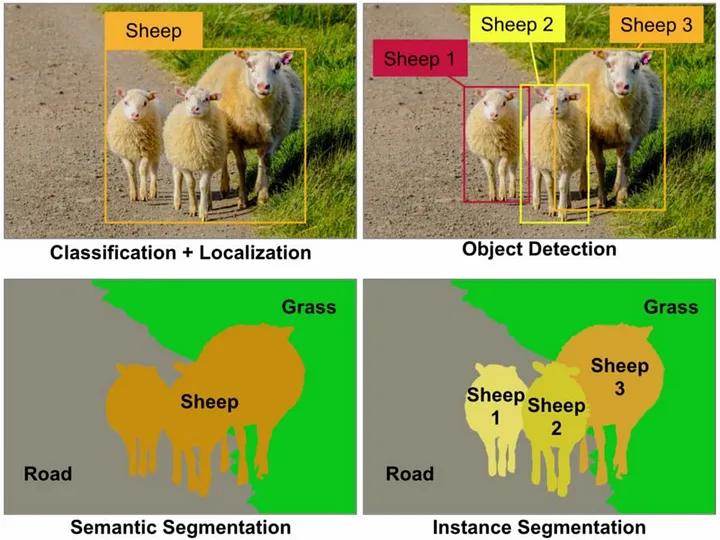
\includegraphics[width=0.75\linewidth]{Images/computer_vision_tasks.png}
    \caption{Computer Vision Tasks (\cite{mu2021object_detection_operations}).}
    \label{fig:computer_vision_tasks}
\end{figure}

The choice of a machine learning model training dataset is reliant on the specific task to be performed. It must contain data suited for that task. For instance, applications tasked with person reidentification require a dataset that includes the identities across images for the persons depicted in the images. An appropriate dataset for such applications, the Person Reidentification in the Wild (PRW), is detailed in Section \ref{sec:dataset_PRW}. A dataset for object detection purposes needs the bounding box and class id for each identified object in the image. In the case of single-class object detection (person localization), only the bouding boxes for each detection for each image would suffice.

\paragraph{Light Conditions in Aquarium Settings}
\phantomsection
\label{sec:scope_aquarium_light}
The environmental conditions within aquarium settings impose specific lighting requirements that significantly influence the deployment and performance of the proposed object detection system. Aquariums typically maintain low-light conditions, presumably to minimize stress for the aquatic animals and improve vision into the tanks for the visitors. In this context, the options for enhancing illumination are often limited, making it impractical to simply increase lighting to facilitate better visual detection technologies. These subdued lighting conditions were an important feature of the thesis project.

\paragraph{TinyML and Frugal Devices}
\phantomsection
\label{sec:scope_tinyML}
An initial attempt was made to encompass tinyML and frugal devices in the project. TinyML is when machine learning models are aimed at deployment to heavily resource-constrained environments, e.g. "frugal devices". These are devices where the microcontroller units (MCUs) are accompanied by memory measured in kilobytes, and processor speeds measured in megahertz. Machine learning networks applied to tiny robots are subject to challenges from size, weight, area, and power (SWAP) (\cite{ne2022robotstinymlconstraints}). Many of the same challenges apply even in applications where the SWAP challenges are not the main concerns. \citeauthor{ra2023reformabletinyml} mentions the open challenges and future directions of the next generation tinyML. Catastrophic forgetting, which is when information from previous tasks while learning new ones are forgotten, are a result of the frugal devices' computational resources and memory\footnote{Catastrophic forgetting can also be seen in transfer learning, and is why freezing the backbone of a pre-trained model may be a good idea.}. The first recommendation for future directions from the authors is to investigate fog computing as a means to offload tasks from the frugal devices. Exploring a system of frugal devices for obtaining sensor data on the edge and "fog devices"\footnote{Fog devices is an unofficial term for processing-instances located close to the edge.} for processing of the data would be a time-consuming objective, especially in a real-world scenario where security must be taken seriously. Therefore, tinyML and frugal devices are not elaborated in detail in this thesis, but discussed briefly in \ref{app:tinyML}. 

\paragraph{Model Hyperparameter Tuning}
\phantomsection
\label{sec:scope_hyperparameter_tuning}
The project did not encompass hyperparameter tuning of the models. Hyperparameter tuning is the process of finding the best hyperparameters for a machine learning model. Hyperparameters are the settings of the model that are not learned from the data, such as the learning rate, batch size, and number of epochs. Hyperparameter tuning is a crucial step in the machine learning pipeline, as it can significantly impact the model's performance. However, due to time and resource constraints, hyperparameter tuning was not included in this project. Further comments on hyperparameter tuning are made in Section \ref{sec:hyperparameter_tuning}.

\paragraph{Person Localization System vs Alternative Notations}
In this thesis, the term \textit{person localization system} is employed consistently to describe the technology developed for identifying the positions of individuals. This terminology is preferred as it aligns with the object detection dataset standards where \textit{person} is the designated class name used in object detection model datasets. Furthermore, the choice of "localization" over "positioning" is deliberate to avoid potential confusion; while "positioning" could imply the physical movement or arrangement of persons by the system, "localization" specifically refers to the precise identification of a person's location within a predefined spatial context, accurately reflecting the capabilities and functionality of the implemented system. Additionally, other literature seems to prefer localizatoin over positioning (\cite{gao2016development}), altough similar systems have also been called indoor \textit{positioning} systems.

\subsection{Disclaimers}
\label{sec:disclaimers}
\subsubsection{Reuse of Previous Work by the same Author}
\phantomsection
\label{sec:disclaimer_reuse}
Some of the subsections in the Literature section are heavily based on an unpublished\footnote{The preliminary study is not publicly available, since this is not the default practice of NTNU.} preliminary study for the project of this thesis by the same authors. This preliminary study was written the semester before, and was a theoretical study of how one may achieve "Efficient, accurate, and privacy-preservant object detection in edge devices" (which was its title). This subsections most influenced by the previous work are the subsections \ref{sec:individual_privacy}, \ref{sec:object_detection}, and \ref{sec:thirdparty_products}.

\subsubsection{The Use of AI Tools}
OpenAI's ChatGPT-4/ChatGPT-4o (\cite{openai2024chatgpt}) has been prompted with several sections to get suggestions on how to enhance readability and flow. All AI generated suggestions have been verified and major parts rewritten to better fit the intentions of the sections. The author of this thesis takes full responsibility for all of its content. ChatGPT was also used to identify typos in the text, as a final step in the production of this thesis.

\subsubsection{Privacy of Similar Projects}
The author of this thesis is not an expert in privacy. The methods outlined in this thesis are meant to ensure privacy of individuals, but the author cannot guarantee that the methods are foolproof. The author has tried to follow best practices and guidelines from the field and has tried to be transparent about the methods used and the limitations of the methods, but the reader should be aware that following the methods outlined in this thesis may not necessarily be enough to ensure privacy. An investigation into the privacy of similar projects is recommended before deploying a similar system in a real-world setting.

\subsection{Research Questions}
\label{sec:research_questions}
Rather than forming a single hypothesis for this rather widespread project, a set of research questions are formulated to guide the research and to provide a structured approach to the investigation.

% The hypothesis of the thesis is that the dataset quality will have an impact on fine-tuned model accuracy, and that the deployment-specific test data will rank the models similarily to the ranking we see on the general datasets. todo hypothesis her bladnes entall og flertall... bestemt/ubestemt..Kanskje del av secondary objectives?

\textbf{The Research Questions are as follows:}
\begin{enumerate}
	\item What are some privacy risks associated with traditional person localization systems in public spaces, and how may a system mitigate these privacy concerns?
	\item How does the validity of object detection model evaluations change when using data specifically from the intended deployment environment compared to using generic datasets?
	\item What are some machine learning architectures suitable for object detection in a real-world deployment scenario?
	\item How do the performance metrics of object detection models compare when applied to different quality datasets?
\end{enumerate}

\subsection{Research Objectives}
\label{sec:research_objectives}
\textbf{The Primary Objectives are to:}
\begin{enumerate}
	\item Develop a privacy-preserving person localization system using on-device processing to minimize data transmission and enhance data privacy.
	\item Demonstrate feasibility and effectiveness of on-device person localization in a practical and realistic setting.
	\item Investigate how the quality of the dataset used in model fine-tuning impacts performance.
	\item Assess the impact of using real world-specific test data on the evaluations of object detection models, by comparing model evaluations obtained with specific test data to evaluations obtained with more general datasets.
\end{enumerate}

\textbf{The Secondary Objectives are to:}
\begin{enumerate}
	\item Compare the privacy and performance impacts of on-device processing against centralized processing methods.
	% \item Investigate the feasibility of deploying the developed system in other public spaces to enhance visitor analytics.
	\item Demonstate how to visualize object detection data by creating visualizations of collected data from a realistic setting.
	\item Explore relevant object detection architectures to evaluate their performance in a real-world deployment scenario.
\end{enumerate}

\subsection{Project Work}
\label{sec:action_points}
\textbf{In order to achieve these objectives, the following project work was executed and is detailed in this thesis:}
\begin{itemize}
    \item Designed and implemented a prototype system that incorporates on-device processing for privacy-preserving person localization.
    \item Deployed a prototype in an aquarium to gather real-world data and analyze system performance.
    \item Collected and labeled a dataset of 3394 images to evaluate and fine-tune several object detector machine learning models.
    \item Conducted comparative studies to evaluate the effects of data specificity and quality on model accuracy.
    \item Performed a comparative analysis of three object detection architectures under real-world conditions.
    \item Developed and utilized advanced visualization tools to represent data findings in a way that facilitates clear understanding and decision-making.
\end{itemize}

This thesis compiles and structures literature on various aspects of person localization systems, bridging multiple domains. It contributes to the field by serving as a collaborative and communicative tool, fostering common understanding among technologists, ethicists, policymakers, and the public.

\subsection{Structure}
\label{sec:structure}
The thesis is structured the following way. The descriptions include what each section will cover and why, to increase readability and coherence of the thesis.

\paragraph{Section \ref{sec:literature}: Literature Review} 
The theoretical underpinnings of the project are surveyed and discussed in the literature review. This section contains text from previous work by the same authors (see \ref{sec:disclaimer_reuse}). The literature review covers a wide range of topics crucial to the development and implementation of on-device processing systems for person localization in environments like museums and aquariums. The following paragraphs provide a summarized overview of the key areas discussed.

Section \ref{sec:visitor_behaviuor_analysis} is included to investigate the need for a person localization system in cultural institutions. The review explores alternative, cost-effective methods for visitor behaviour analysis already on the market such as mobile apps and RFID tracking. These technologies provide scalable solutions without the privacy concerns associated with vision-based systems. Museum stakeholders opinions are included in this section. This section presents insights into user perceptions of privacy in smart home environments, which reveal a trade-off between convenience and privacy concerns, indicating similar challenges could arise in public visitor contexts. Section \ref{sec:GDPR} about GDPR seek to illustrate how these challenges are addressed in the current EU regulations. It summarizes the requirements for personal data protection and the legal bases for processing such data, which are directly applicable to any person localization system developed. Together with the NIS2 directive, the GDPR promotes the principle of data minimization, pushing for a solution that deletes unnecessary data as soon as the data is redundant.

Section \ref{sec:individual_privacy} provides an in-depth overview of some of the approaches and methods to preserve privacy, specifically in images. The review delineates the privacy advantages of on-device processing over cloud-based systems, emphasizing the importance of local data processing to mitigate privacy risks. Exploration of technologies like federated learning and differential privacy illustrates advanced methods for protecting individual privacy while utilizing data for machine learning. 

Section \ref{sec:ethics_localization_tech} presents some various opinions and ethical considerations related to person localization technologies. These perspectives come from a former developer in the field of object detection, an acclaimed writer, and multiple philosophers. 

Section \ref{sec:object_detection} provides a technological overview of object detector datasets, performance metrics, object detector algorithms, dark-lit environment considerations, and transfer learning. The descriptions for the algorithms are relatively short altough they are important, as the most accurate descriptions are found elsewhere. A subsection of the key differences and similarities between the object detector algorithms of this thesis project are included. Section \ref{sec:thirdparty} and Section \ref{sec:thirdparty_products} brings forth various third party software services and products. These are included due to their relevancy to the project of this thesis and to improve awareness around potential already-existing implementations that may fit a given use case. Specifically, Roboflow and GPT-4 with Vision are evaluated for their utility in building and deploying person localization systems, with considerations on their implications for privacy and data security in real-world applications. Finally, several options for relevant hardware are presented in Section \ref{sec:hardware_options}. This includes microcontrollers and single board computers, specialized components such as graphical-, tensor-, and neural processing units (GPUs, TPUs and NPU), and various sensors capable of relevant functionalities.

\paragraph{Section \ref{sec:methodology}: Methodology}
The Methodology section outlines the detailed technical approaches and methods employed in this project. This section is critical for understanding how the data was collected, processed, and analyzed. It provides a foundation for interpreting the results and findings of this thesis, and a common understanding of the terms.

Section \ref{sec:project} provides an overview of the project, including the hardware decisions and the deployment of devices in the aquarium. This section also explains the different machine learning models employed for training and evaluation. Section \ref{sec:dataset_construction} delves into the construction of the \textit{FIMUS} dataset. It covers the camera configurations, image capturing process, and labeling. This section highlights the differences between the inconsistent and consistent partitions of the dataset, detailing the specific settings and processes used to ensure the quality and relevance of the captured images. Section \ref{sec:external_datasets} briefly describes the external datasets used in the project; COCO, CrowdHuman, Person Reidentification in the Wild, and Football-players. It explains the relevance of each dataset to the project and how they were utilized for model training and evaluation.

Section \ref{sec:model_training} focuses on the training process of the models. The section contains information regarding the licenses of the models, and the hyperparameter tuning process (which was mostly foregone), and the use of Google Colab for cloud training with GPUs, detailing a few pros and cons. Finally, it provides an explanation regarding the lack of validation used in the training of the models, a decision based both on the lack of hyperparameter optimization in the project and issues with google colab service disconnections. 

Section \ref{sec:methodology_model_evaluation} restates the metrics used to evaluate the performance of the models in this thesis project, and defines them as \textit{COCO AP} and \textit{Vary-Both AP}. Section \ref{sec:model_presentation} presents the different models that were developed and tested in the project. It includes details about the pre-trained and fine-tuned models, their configurations, and the specific experiments conducted to measure their performance.

Section \ref{sec:ethics_localization_tech} addresses the ethical methodologies that were implemented in the project to ensure preservation of privacy. Section \ref{sec:heatmaps} discusses the use of heatmaps as a visualization tool to analyze visitor behavior patterns. It details the attempts to create heatmaps using different Python packages and the final implementation using the Supervision module by Roboflow\footnote{A final heatmap is displayed in the end of this section, and in the results (Section \ref{sec:data_visualization})}.

By following this structure, the Methodology section provides a comprehensive and transparent account of the technical processes involved in the project, ensuring that the results are reproducible and the conclusions are drawn based on a solid and well-documented foundation. 

\newpage
\paragraph{Section \ref{sec:results}: Project Results} 
This section presents the findings and performance evaluations of the person localization system implemented in the project. It includes detailed experiments designed to address the research questions and objectives outlined in Section \ref{sec:research_questions}, highlighting their implications and significance within the broader context of the field.

Section \ref{sec:object_detection_model_evaluation} evaluates the object detection models using various dataset partitions and presents the results of different experimental setups. It includes a detailed analysis of average precisions and recalls, and explores the effects of fine-tuning, different test-set compositions, and input image sizes on model accuracy and inference latency.

Section \ref{sec:data_visualization} discusses the visualization of data through heatmaps and peak hours analysis, providing insights into visitor behavior patterns and engagement levels. Subsections illustrate how heatmaps and bar charts are used to analyze and visualize the data, highlighting visitor engagement patterns and identifying peak visitation times.

By presenting these results, this section provides a comprehensive overview of feasibility and effectiveness of a person localization system. It also serves as a demonstration of the practical implications and potential applications of the person localization system in a real-world setting.


\paragraph{Section \ref{sec:reflections}: Reflections \& Overall Discussions} 
This section provides a comprehensive discussion of the broader implications of the research findings, reflecting on the results and their significance for the development of similar systems. It evaluates the viability of the approach used in this thesis to address the presented problem and restates the research questions from the introduction, providing concrete answers to each.

Section \ref{sec:privacy_in_images} discusses the privacy implications of image deletion versus obfuscation post-analysis. It critiques existing studies on privacy preservation and argues for the need to consider demographic and cultural differences in privacy perceptions.

Section \ref{sec:discuss_thirdparty} examines the use of third-party services and products, highlighting potential drawbacks such as loss of control, data privacy concerns, cost efficiency, performance optimization, and scalability issues. It emphasizes the importance of balancing the convenience of third-party solutions with the need for customization, security, and long-term cost management.

Section \ref{sec:discussion_ethics_localization_tech} explores the ethical considerations of developing person localization systems. It discusses the potential risks of mass public control and the importance of ethical frameworks such as utilitarianism and deontological ethics in evaluating the impacts of these technologies. The section underscores the need for rigorous ethical assessments and informed regulation to ensure the responsible deployment of person localization technologies.

Section \ref{sec:hardware_choices} reflects on the hardware and software choices made in the project, considering their adequacy and potential areas for improvement. It discusses the benefits and limitations of using Python for on-device processing and suggests considerations for optimizing device efficiency with lower-level programming languages.

Section \ref{sec:results_discussion} summarizes the results of the project, comparing COCO AP and Vary-Both AP metrics and discussing their implications for model selection. It highlights the importance of balancing precision and recall in evaluating object detection models and the need for comprehensive performance metrics.

Section \ref{sec:discussion_research_q} provides concise answers to the research questions posed at the beginning of the thesis, summarizing the findings and their implications. It addresses privacy risks, the validity of model evaluations using specific datasets, suitable machine learning architectures, and the impact of dataset quality on performance metrics.

\newpage
Section \ref{sec:discussion_broader_context} situates the project within a broader context by discussing its implications for public environment deployment, privacy preservation, and the applicability of object detection models in various settings. It emphasizes the practical utility of the system for crowd management and operational efficiency, and highlights the essential ethical considerations for deploying such technologies in public spaces. The project demonstrates the feasibility and effectiveness of on-device person detection in realistic settings, providing valuable insights into model performance and adaptability, while underscoring the importance of thoughtful and comprehensive ethical standards in technology development.

\paragraph{Section \ref{sec:future_work}: Future Work}
This section outlines a comprehensive research agenda to advance on-device person detection systems, building on the findings of this thesis. It addresses remaining questions and proposes several future research directions. These include evaluating fine-tuned models on generic datasets to assess their generalizability and robustness across diverse environments, expanding the FIMUS dataset to create a more diversified person localization dataset, and exploring advanced privacy-preserving techniques such as differential privacy and homomorphic encryption.

Further, it proposes expanding practical applications of on-device detection technologies to areas such as smart home automation, healthcare monitoring, and personalized user experiences in public venues. Enhancing data visualization tools by integrating additional variables for heatmap generation and creating zones to visualize visitor flow and exhibition popularity are also recommended.

These propositions aim to guide future research, ensuring the continued development and ethical deployment of on-device person detection systems.

\paragraph{Section \ref{sec:conclusions}: Conclusions} 
This section summarizes the key insights and findings of the thesis, concluding the research on the viability and ethical implications of on-device person detection systems. It encapsulates the significance of privacy preservation, the importance of relevant datasets for model evaluation, and the ethical considerations essential for responsible technology deployment. The conclusion also reflects on the practical implementation, future research directions, and policy recommendations, providing a comprehensive closure to the thesis.

\paragraph{Appendix A: Code Snippets} Appendix A provides guidance on the sequence for setting camera configurations to achieve consistent image quality for the dataset, detailed in Table \ref{tab:picamera_settings}. It emphasizes the importance of setting the shutter speed first and allowing the automatic gain control to stabilize before disabling automatic settings and manually adjusting the white balance gains.

\paragraph{Appendix B: Camera Settings Explanation} This is a quick and easy-access overview for understanding the camera module settings that were used in this project. 

\paragraph{Appendix C: TinyML and Frugal Devices} This appendix spans 4 paragraphs which landed outside the scope of the project, but is included for its relevancy for similar systems with lower complexity hardware. 

\paragraph{Formatting Guidelines}
This document adheres to APA formatting guidelines for quotations, by indenting block quotations longer than 40 words and enclosing shorter quotations within the text in quotation marks. Page numbers are excluded due to the efficiency of digital search tools. Title case capitalization is applied to section headings (also in line with APA style).

% \newpage
% \subsubsection{APA-Format}
% In accordance with APA-style, 
% \begin{itemize}
% 	\item Every quotation of over 40 words has been formatted as a free-standing block without quitation mark. These blocks are indented (\cite{UCR2024}). 
% 	\item Quotations of fewer than 40 words are included in the text and surrounded with quotation marks. The page number has not been included as it is considered irrelevant with todays digital tools as one may search for the exact sentence instead and find it much faster.
% 	\item The sections and subsections within implement title case capitalization in accordance with APA-style (\cite{apa_title_case}). 
% \end{itemize}